\chapter{Continuous Integration}
Continuous Integration is geregeld door TravisCI, voor open source projecten is TravisCI gratis te gebruiken.
Omdat het project met Gradle is gebouwd is het makkelijk om CI ondersteuning toe te voegen aan de backend.
Het commando "gradle test" draait alle tests in het project, als er iets fout gaat is dit ook meteen in Github zichtbaar.

\begin{figure}[H]
	\includegraphics[width=\textwidth]{images/TravisCi.png}
	\caption{Overzicht TravisCI}
	\label{fig:TravisCI}
\end{figure}
Travis is ook private te gebruiken, dit zorgt ervoor dat je meer jobs tegelijk kunt draaien.
Hoe meer je betaald, hoe meer jobs je kan tegelijktijd kan gebruiken.
Iedereen krijgt wel unlimited build minutes, repositories en collaborators.

Travis CI kan geconfigureerd worden met een bestand dat .travis.yml heet, dit bestand is zoals te zien in .yml formaat.
Dit bestand moet in de root van je project geplaatst worden. 
\begin{figure}[H]
	\centering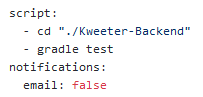
\includegraphics[width=0.33\textwidth]{images/TravisCIYml}
	\caption{TravisCI Yaml}
\end{figure}

Het bovenstaande script zorgt ervoor dat gradle tests automatisch worden uitgevoerd.
Het TravisCI script wordt uitgelezen en uitgevoerd op een Ubuntu server van Travis.
De output van dit script kan ook uitgelezen worden op de website, dit zorgt ervoor dat je kan kijken hoe je tests draaien, en eventueel de oorzaak van errors kan vinden.

TravisCI draait je scripts automatisch bij elke commit die naar Github wordt gemaakt, en het resultaat is binnen een minuut zichtbaar.